\documentclass[10pt]{article}\usepackage[margin=.55in]{geometry}\usepackage[T1]{fontenc}\usepackage{graphicx}\setlength{\parindent}{0pt}\setlength{\parskip}{5pt}\sloppy\begin{document}{\large Private runtime qualifier source}\par Task T-1417. 3 November 2026.\par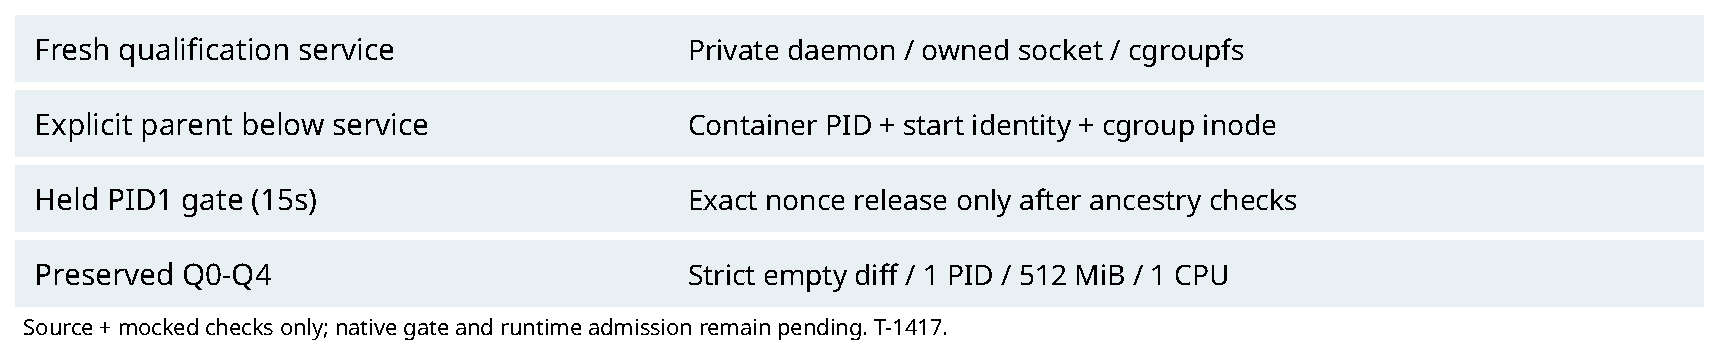
\includegraphics[width=\linewidth]{diagram.pdf}\par A concrete copied qualifier now routes both Docker CLI and curl archive metadata through one pinned private UNIX socket. It requires the private daemon ID and cgroupfs driver, passes an explicit container cgroup parent below the bounded service, and verifies host PID lifetime, strict ancestry and gate/host cgroup inode correspondence before releasing tested execution.

The original gate immediately execed after its receipt. The new source adds a bounded 15-second no-fork nonce-release wait on existing /work tmpfs, with effective PID checks after release. Only complete exact root-owned 0444 token bytes release; partial archive extraction or wrong tokens cannot exec and remain bounded by the same deadline. The original gate and qualifier remain unchanged. The final success guard rejects pending signals and expired monotonic/UTC limits.

Validation is source and mocked software validation: 12 Python tests pass, including endpoint mismatch, wrong ownership, sibling-prefix containment, socket replacement, PID reuse, cgroup inode/PID-limit mismatch, release ordering/failclosed denial, final signal/deadline boundaries and static original-control/gate ordering checks. No native gate compilation/control execution, Docker, sudo, systemd, container or cloud invocation occurred. The gate partial-write behavior has source/static checks; its native controls remain pending in native-gate-controls-pending.json.

Preserved controls: Q0-Q4, fixed owner digest, fixture and gate reviews, head\_contract.py binding, strict empty diff, one container, 512 MiB memory, 1 CPU and 1 PID, restricted mounts/capabilities/namespaces, 300-second qualification ceiling including 30-second cleanup reserve and 20-second active cases. No empty-diff exception is added for the gate mount; that remains a runtime qualification condition.

Supervisor interface: separate 600-second assembly and 300-second qualification services, no live daemon reuse. Qualification uses retained disk only after predecessor shutdown/empty-cgroup custody, plus a fresh qualification endpoint and source/image/input/assembly receipt joins. INTERFACE.md lists exact fields and callback arguments. The callback must inherit the bounded service and INVOCATION\_ID, and the private cgroup parent must be empty and delegated.

Source evidence: preserved runtime-qualifier-v5, preexec-native-controls-v2/gate.c, and installed primary Docker create/dockerd and systemd.resource-control manuals; exact hashes in source-provenance.json. These establish the explicit parent and delegation interfaces; no live containment conclusion follows from documentation alone.

Draft admission remains false; final image, new held-gate binary/control evidence, independent gate/source review and runtime qualification remain required. The planning limit 25,200 active-worker seconds through 2026-11-04T06:00:00Z does not admit execution. Canonical scientific plots remain unchanged; this report concerns the new source interface and its mocked checks.
\end{document}